% Manual for ForwardCom softcore model A

\documentclass[11pt,a4paper,oneside,openright]{report}
\usepackage[bindingoffset=5mm,left=20mm,right=20mm,top=20mm,bottom=20mm,footskip=10mm]{geometry}
\usepackage[utf8x]{inputenc}
\usepackage{hyperref}
\usepackage[english]{babel}
\usepackage{listings}
\usepackage{subfiles}
\usepackage{longtable}
\usepackage{multirow}
\usepackage{ragged2e} 
\usepackage{amsthm} % example numbering
\usepackage{color}
\usepackage[T1]{fontenc} % fix problem with underscore not searchable
\usepackage{fontspec}
\usepackage{caption}
\usepackage{graphicx}
\defaultfontfeatures{Mapping=tex-text, Ligatures=NoCommon}
\setmainfont{Arial}[Ligatures=NoCommon]
\setsansfont{Arial}
\renewcommand{\familydefault}{\sfdefault}

% modify style
\newtheorem{example}{Example}[chapter]  % example numbering
\lstset{language=C}                     % formatting for code listing
\lstset{basicstyle=\ttfamily,breaklines=true}
\definecolor{darkGreen}{rgb}{0,0.4,0}
\lstset{commentstyle=\color{darkGreen}}
\captionsetup{justification=raggedright,singlelinecheck=false}

\newcommand{\vv}{ \vspace{2mm} }   % vertical space


\begin{document}
\title{ForwardCom softcore model A}
\author{Agner Fog}
\date{\today}
\maketitle
\RaggedRight

\tableofcontents
\setcounter{secnumdepth}{1}


\chapter{Introduction}
ForwardCom is a new instruction set architecture with corresponding hardware and software standards. An introduction to ForwardCom can be found at the website \href{https://www.forwardcom.info}{www.forwardcom.info}. 
A full description and definition is found in the manual 
\href{https://github.com/ForwardCom/manual/raw/master/forwardcom.pdf}{ForwardCom: An open-standard instruction set for high-performance microprocessors}.
\vv

The present document describes the softcore model A 
for implementing a ForwardCom CPU in a Xilinx Artix-7 FPGA.
\vv

\subsection{Features of model A version 1.01}
\begin{itemize}
\item Runs on Nexys A7-100T FPGA board
\item Maximum clock frequency 50 - 70 MHz, depending on configuration
\item 32-bit or 64-bit registers
\item Can execute one instruction per clock cycle
\item Data memory 32 kB. Code memory 64 kB. Call stack 1023 entries.
\item Implements all integer instructions, including advanced and complex instructions
\item Implements all instruction formats and all addressing modes defined by the ForwardCom standard version 1.12.
\item No vector registers. No floating point instructions
\item No system calls, no memory protection. Useful for embedded designs
\item Memory reads and writes must be aligned
\item RS232 serial interface for standard input and output
\item On-chip loader (uses 1 kB code memory)
\item On-chip debug interface
\item On-chip event counter
\item Code examples and test suite provided
\end{itemize}
\vv

\subsection{Prerequisites}
\begin{itemize}
\item FPGA board Digilent Nexys A7 100T or Nexys 4
\item Xilinx Vivado tools version 2020.1
\item ForwardCom softcore
\item ForwardCom binary tools "forw" version 1.12 or later
\item Serial terminal program, such as RealTerm or Tera Term
\item Windows or Linux PC
\end{itemize}
\vv


\chapter{Getting started} \label{Chap:GettingStarted}
The softcore is available at 
\href{https://github.com/ForwardCom/softcoreA}{github.com/ForwardCom/softcoreA}. \\

Device-specific files for The Nexys A7-100T FPGA board are provided in 
\href{https://github.com/ForwardCom/softcoreA/tree/main/deviceA7100T}{the subfolder deviceA7100T}. \\


\begin{itemize}
\item Install Vivado version 2020.1. If you are using a later version, make sure that it supports Artix 7 series FPGAs
\item Get the softcore project zip file A1.xpr.zip and unpack it. Open the project file A1.xpr with Vivado.
\item In Vivado, go to the Flow Navigator window and open Hardware Manager
\item Connect the FPGA board to the PC with the USB cable that comes with the board. Turn on the FPGA board on the slide switch on top. You will see a moving pattern on the display. Install the FTDI driver on the PC if it does not install automatically.
\item In Vivado Hardware Manager, click Open target -> Auto Connect. (If connection fails, restart the computer and use a different USB port).
\item Click Program device, and select the file \{my directory\}/A1/A1.runs/impl\_1/top.bit \\
You will see numbers on the display
\item Now you can upload a program to the soft core CPU. Choose hello.ex as a start. Upload this file in binary mode to the virtual serial port that corresponds to the USB port. Use 230400 Baud, 8 data bits, 1 stop bit, no parity, no flow control. 
The BAUD rate can be changed in the file configXXX.vh. 
The following describes how to do the uploading with a terminal program:
\item If you are using RealTerm: \\ 
Open RealTerm. On the Display tab, choose Display as All Chars, newLine mode. \\ 
On the Port tab, set Baud = 230400. In the Port field, find the port number that corresponds to the USB connection. In my case, it shows 4=VCP0, but it may have a different number on your computer. The number may change if you use a different USB port. Press the Open button twice to close the connection and open again. Look at the Status to the right and make sure it is not Closed.\\
Go to the Send tab. Set checkmarks in "+LF" in the first two lines. Set delays to 0. Under "Dump file to port", find the file you want to upload (hello.ex) and press Send. (If you want to upload again, press the "cpu reset" button on the FPGA board to activate the loader).\\
Press the Up button on the FPGA board if the program asks you to press Run. The hello.ex program writes a welcoming text on the terminal.
\item If you are using Tera Term: \\ 
On New Connection, click Serial. In the Port window, choose USB Serial Port. \\
Click on the Setup menu -> Serial Port. Set speed = 230400, and click New Setting\\
In the File menu -> Send file. Set Option = Binary. Open the file hello.ex \\
Press the Up button on the FPGA board to start the program. You should see a Hello text on the terminal.
\item If you are using Linux: \\ 
I have not tried this on Linux yet. You need a serial terminal program that can transfer files.
\end{itemize}


\chapter{Examples and test programs}
Some code examples are available as assembly code at \\
\href{https://github.com/ForwardCom/code-examples}{github.com/ForwardCom/code-examples}.
\vv

The same examples compiled for the softcore are available as .ex files at \\
\href{https://github.com/ForwardCom/softcoreA/tree/main/deviceA7100T}{github.com/ForwardCom/softcoreA/tree/main/deviceA7100T}.
\vv

The following examples work on the softcore model A:
\begin{itemize}
\item hello.ex: Write a welcoming message on the serial terminal
\item calculator.ex: Enter two integers a, and b. The program will calculate a+b, a-b, a*b, a/b, and a modulo b.
\item guess\_number.ex: A guessing game. The user has to guess a random number. The program tells if the number is bigger or smaller than your guess.
\end{itemize}

These examples are compiled from the assembly code and the libc\_light.li function library. Upload one of the .ex files as described above to run these examples on the softcore, 
\vv

The same examples can run on the emulator when linked with libc.li instead of libc\_light.li.

\subsubsection{Test suite}
A test suite is provided for testing all instructions and formats. The source code for the test programs are available at:\\

\href{https://github.com/ForwardCom/test-suite}{github.com/ForwardCom/test-suite}
\vv

The same test programs compiled for the softcore are available as .ex files at \\
\href{https://github.com/ForwardCom/softcoreA/tree/main/deviceA7100T}{github.com/ForwardCom/softcoreA/tree/main/deviceA7100T}.
\vv

The following test programs work on the softcore model A:
\begin{itemize}
\item tests\_arithmetics.ex: Test all integer arithmetic instructions
\item tests\_bool\_bit.ex: Test all boolean and bit manipulation instructions
\item tests\_branch.ex: Test all jump, call, and branch instructions
\item test\_formats.ex: Test all instruction formats
\item test\_pipeline\_stalls.as: Test synchronization and stalls in pipeline
\item test\_muldiv.as: Test multiplication and division
\item testpushpop.as: Test push and pop instructions
\end{itemize}
\vv

The 32-bit version of the softcore obviously fails the tests on 64-bit operands.
\vv


\chapter{User interface}
The FPGA board is connected to a PC through a USB cable. Standard input and output are provided as an RS232 serial connection tunneled through the USB cable with an FTDI driver installed on the PC. A terminal program running on the PC may be used for user input and output. The transmission parameters are 230400 Baud, 8 data bits, 1 stop bit, no parity, no flow control, 
\textbackslash{LF} as line feed. The Baud rate can be changed by modifying a configuration file (see page \pageref{SettingConfiguration}) and rebuilding the hardware code.
\vv

The pushbuttons on the FPGA board are used as follows:
\vv

\begin{tabular}{|l|l|} 
\hline
\bfseries Operation  & \bfseries Use pushbutton  \\ \hline
Run  &  $\uparrow$  \\ \hline
Single step  &  $\rightarrow$  \\ \hline
Restart  &  $\downarrow$  \\ \hline
Load program  &  CPU reset  \\ \hline
\end{tabular}
\vv

The Run button will make the program run if it has stopped at a breakpoint. Test programs and examples often start with a breakpoint so that they will run only when you press the Run button.
\vv

The Single step button allows you to execute CPU instructions one by one for debugging purposes. See chapter \ref{Chap:Debugger}
\vv

The Restart button makes the program restart from the beginning. All registers are reset, but static data are not reset.
\vv

The Load program button lets you load a new program. Press the Load program button and send a new .ex file from the terminal program, as explained on page \pageref{Chap:GettingStarted}.
\vv

The pushbuttons on the FPGA board are small and impractical. You may add external pushbuttons as described on page \pageref{Chap:ExternalPushbuttons}.
\vv

Runtime errors are indicated by a flashing LED. The type of error is shown on the LED displays with the following codes:
\vv

\begin{tabular}{|l|l|l|} 
\hline
\bfseries Error code  & \bfseries Error when loading & \bfseries Error when running  \\ \hline
E1  & Error in .ex file & Unknown instruction \\ \hline
E2  & Code size too big & Wrong operands for instruction \\ \hline
E3  & Data size too big & Array index overflow \\ \hline
E4  &  & Memory read violation \\ \hline
E5  &  & Memory write violation \\ \hline
E6  &  & Misaligned memory read or write \\ \hline
\end{tabular}
\vv

The error code is followed by the code address where the error was detected, as a hexadecimal number.
\vv

The LED display shows debugging information when there is no error (no flashing LED). See chapter \ref{Chap:Debugger}
\vv

\chapter{Serial input and output} \label{Chap:SerialIO}

The following port numbers are provided for serial input and output.
\vv

\begin{tabular}{|l|l|l|} 
\hline
\bfseries Port number & \bfseries Function & \bfseries Bits \\ \hline
Input port 8 & serial input & bit 0-7: received byte \\
             & RS232        & bit 8: (Data valid. Unreliable) \\
             &              & bit 9: At least one more input byte is ready \\
             &              & bit 12: Input buffer overflow error \\
             &              & bit 13: Frame error in start bit or stop bit \\ \hline
Input port 9 & serial input status & bit 0-15: Number of bytes in input buffer \\
             &              & bit 16: Input buffer overflow error \\
             &              & bit 17: Frame error in start bit or stop bit\\ \hline
Output port 9 & serial input control & bit 0: Clear buffer. Delete all data in input buffer and clear error status \\
             &              & bit 1: Clear error status but keep data \\ \hline
Output port 10 & serial output & bit 0-7: byte to send \\
              & RS232         & other bits are reserved  \\ \hline
Input port 11 & serial output status & bit 0-15: Number of bytes in output buffer \\
              &              & bit 16: Output buffer overflow error \\
              &              & bit 18: Ready. Output buffer is not full \\ \hline
Output port 11 & serial output control & bit 0: Clear buffer. Delete all data in output buffer and clear error status \\
             &              & bit 1: Clear error status but keep data \\ \hline
\end{tabular}
\vv

The size of the input buffer is 1kB. The size of the output buffer is 2kB. The Baud rate and buffer sizes can be changed in a configuration file (see page \pageref{SettingConfiguration}).
\vv

\chapter{Control registers and performance counters} \label{Chap:ControlRegisters}

The following capabilities registers are supported:
\vv

\begin{tabular}{|c|c|l|} 
\hline
\bfseries Register & \bfseries Read/Write & \bfseries Functionality \\ \hline
capab0 & R   & Microprocessor model = "A" \\ \hline
capab1 & R  & Microprocessor version = 0x10000 \\ \hline
capab2 & RW & Disable error traps \\ \hline
capab4 & R  & Code memory/cache size in bytes \\ \hline
capab5 & R  & Data memory/cache size in bytes \\ \hline

capab8 & R  & Support for operand sizes \\ \hline
capab9 & R  & Support for operand sizes in vectors \\ \hline
capab12 & R & Maximum vector length in bytes \\ \hline
capab13 & R & Maximum vector length for permute instructions \\ \hline
capab14 & R & Maximum block size for permute instructions \\ \hline
capab15 & R & Maximum vector length for compress\_sparse and expand\_sparse. \\ \hline
\end{tabular}
\vv
\vv
\vv

The following performance counters are supported:
\vv

\begin{tabular}{|c|l|} 
\hline
\bfseries Register & \bfseries Functionality \\ \hline
perf1  & CPU clock cycles \\ \hline
perf2  & Number of instructions executed \\ \hline
perf3  & Number of vector instructions executed \\ \hline
perf4  & Vector registers in use \\ \hline
perf5  & Jumps, calls, and return instructions \\ \hline
perf8  & Runtime errors \\ \hline
\hline
\end{tabular}
\vv

The performance counter registers are read-only, but it is possible to reset these registers to zero. 
\vv

Details of these registers are provided in the ForwardCom manual. 
\vv


\chapter{Debugger} \label{Chap:Debugger}
The softcore has two debugging interfaces: A LED display for showing internal signals in the CPU, and an external LCD display for showing the contents of each pipeline stage as well as the result of each instruction.
\vv

Both displays are useful when single-stepping through the code. Set a breakpoint instruction in the assembly code at the point where you want to begin single-stepping. Use the single-step button ($\rightarrow$) to execute instructions one by one. Use the run button ($\uparrow$) to run to the next breakpoint or end of program. It is possible to use external buttons instead of the small pushbuttons on the FPGA board, as described in chapter \ref{Chap:AddOnBoards}. 
\vv

\section{LED display}
The LED display on the FPGA board can show any internal signal in the CPU during single-stepping. The sixteen switches on the FPGA board are used for selecting which signal to view. All signals are shown as hexadecimal numbers on the LED display.
\vv

Switch number 7-4 are selecting which pipeline stage or unit to show, and switch 3-0 are selecting which signal from this stage or unit to show. 
For example, if you set switch 7-0 to 01110000, you can see the pipeline synchronization signals.
\vv

All the possible signals to view are defined in the file debugger.vh. 
You may modify the file debugger.vh to show any signal that is not already defined and assigned to a switch combination. Some signals are commented out in order to economize wiring resources.
\vv

All pipeline stages and units have registers (D-flip flops) at the output, showing the values after one clock pulse. If you want to see an internal signal that is not output through a register from the unit in question, then it is recommended to output this signal through a register before sending it to the debug display. This makes sure that signals are properly synchronized so that you do not see signals that belong to different clock periods at the same time on the display (which can be very confusing). See the output debug1\_out in the file decoder.sv for an example of how to do this.
\vv

The LED display can also show register values. Set switch 8 high and set switch 0-5 to the register number as a binary value. The LED display will show the lower 32 bits of the register as a hexadecimal value on the eight LED display digits. 
Only two digits are shown if the register value is not known but waiting for a value to be calculated by the ALU. The two digits show the tag of the instruction that will provide the value in this case.
\vv

\section{External LCD display}
It is possible to add an external LCD display to show results and how instructions propagate through the pipeline when single-stepping. Instructions for building the external LCD display are given in chapter \ref{Chap:AddOnBoards}.
\vv

The LCD display has eight lines (four on each LCD unit). The eight lines show the contents of the pipelines as follows:
\vv

\begin{tabular}{|l|l|l|} 
\hline
\bfseries Line & \bfseries Symbol & \bfseries Showing  \\ \hline
1  & F & Fetch stage instruction \\ \hline
2  & D & Decode stage instruction \\ \hline
3  & R & Register read stage instruction \\ \hline
4  & A & Address generation stage instruction \\ \hline
5  & d & Data read stage instruction \\ \hline
6  & X & Execute (ALU) stage instruction \\ \hline
7  & : & ALU inputs or mul/div result \\ \hline
8  & = & ALU result \\ \hline
\end{tabular}
\vv

Each pipeline stage is represented by a line showing the code address (lower 16 bits as hexadecimal), instruction format, operand type, and instruction name. See figure \ref{fig:addOnBoard} on page \pageref{fig:addOnBoard}. 
\vv

The operand type is coded with one letter as follows: b=int8, h=int16, w=int32, d=int64, q=int128, F=float32, D=float64, Q=float128.
\vv

Line 7, indicated as ':', shows three hexadecimal numbers representing the lower 16 bits of the values of up to three input operands of the current instruction. The first field shows the first operand of 3-operand instructions, or a fallback value for instructions with less than 3 operands. The second field shows the second operand of 3-operand instructions or the first operand of 2-operand instructions. The third field shows the last operand.
\vv

Line 8, indicated with '=', shows the result of the current instruction as a hexadecimal number (32 bits). 'm0' indicates a mask bit of 0, giving a fallback value. The result of conditional and indirect jump instructions are indicated as 'jump' or 'no jump'.
\vv

Multiplication and division instructions (including mul\_add and rem) have longer latencies so that the results are shown only after a delay of several clock cycles. These results may appear simultaneously with some other instruction. Multiplication and division results are shown in line 7 instead of input operands. 
\vv

Direct unconditional jump, call, and return instructions are only visible on the first line because they are handled by the fetch unit only.
\vv

Pipeline bubbles due to fetch delays, jump delays or stalls in the address generation stage are indicated by '-'.
\vv

Pipeline stalls are indicated by '\#'. This occurs when the address generator stage or the execute stage is waiting for a register value.
\vv


\chapter{Add-on boards} \label{Chap:AddOnBoards}

\subsection{Adding external pushbuttons} \label{Chap:ExternalPushbuttons}
It is convenient to add external pushbuttons to replace the small buttons on the FPGA board. The following components are needed.
\vv

\begin{table}[h]
%\centering
\begin{tabular}{|l|l|} 
\hline
\bfseries Component & \bfseries number  \\ \hline
VERO board or similar & 1 \\ \hline
Pushbutton, for example Digitast & 4 \\ \hline
2x6 pin male connector & 1 \\ \hline
Resistor 10 k\Omega & 4 \\ \hline
\end{tabular}
\caption{Component list for external pushbuttons}
\label{table:ComponentListPushbuttons}
\end{table}
\vv

The pushbuttons can be connected to the JB socket on the FPGA board according to this diagram:

\begin{center}
\begin{figure}[ht]
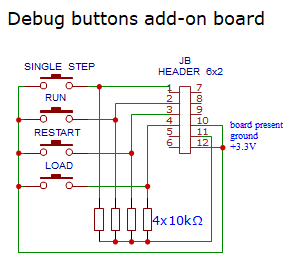
\includegraphics{SchematicDebugButtons.png}
\caption{Circuit diagram for connecting external pushbuttons}
\label{fig:PushbuttonsDiagram}
\end{figure}
\end{center}
\vv

An add-on board with both LCD display and pushbuttons is shown in figure  \ref{fig:addOnBoard}. The buttons on the photo are: Black: single step, Green: run, Red: restart, Blue: load.
\vv

\begin{center}
\begin{figure}[ht]
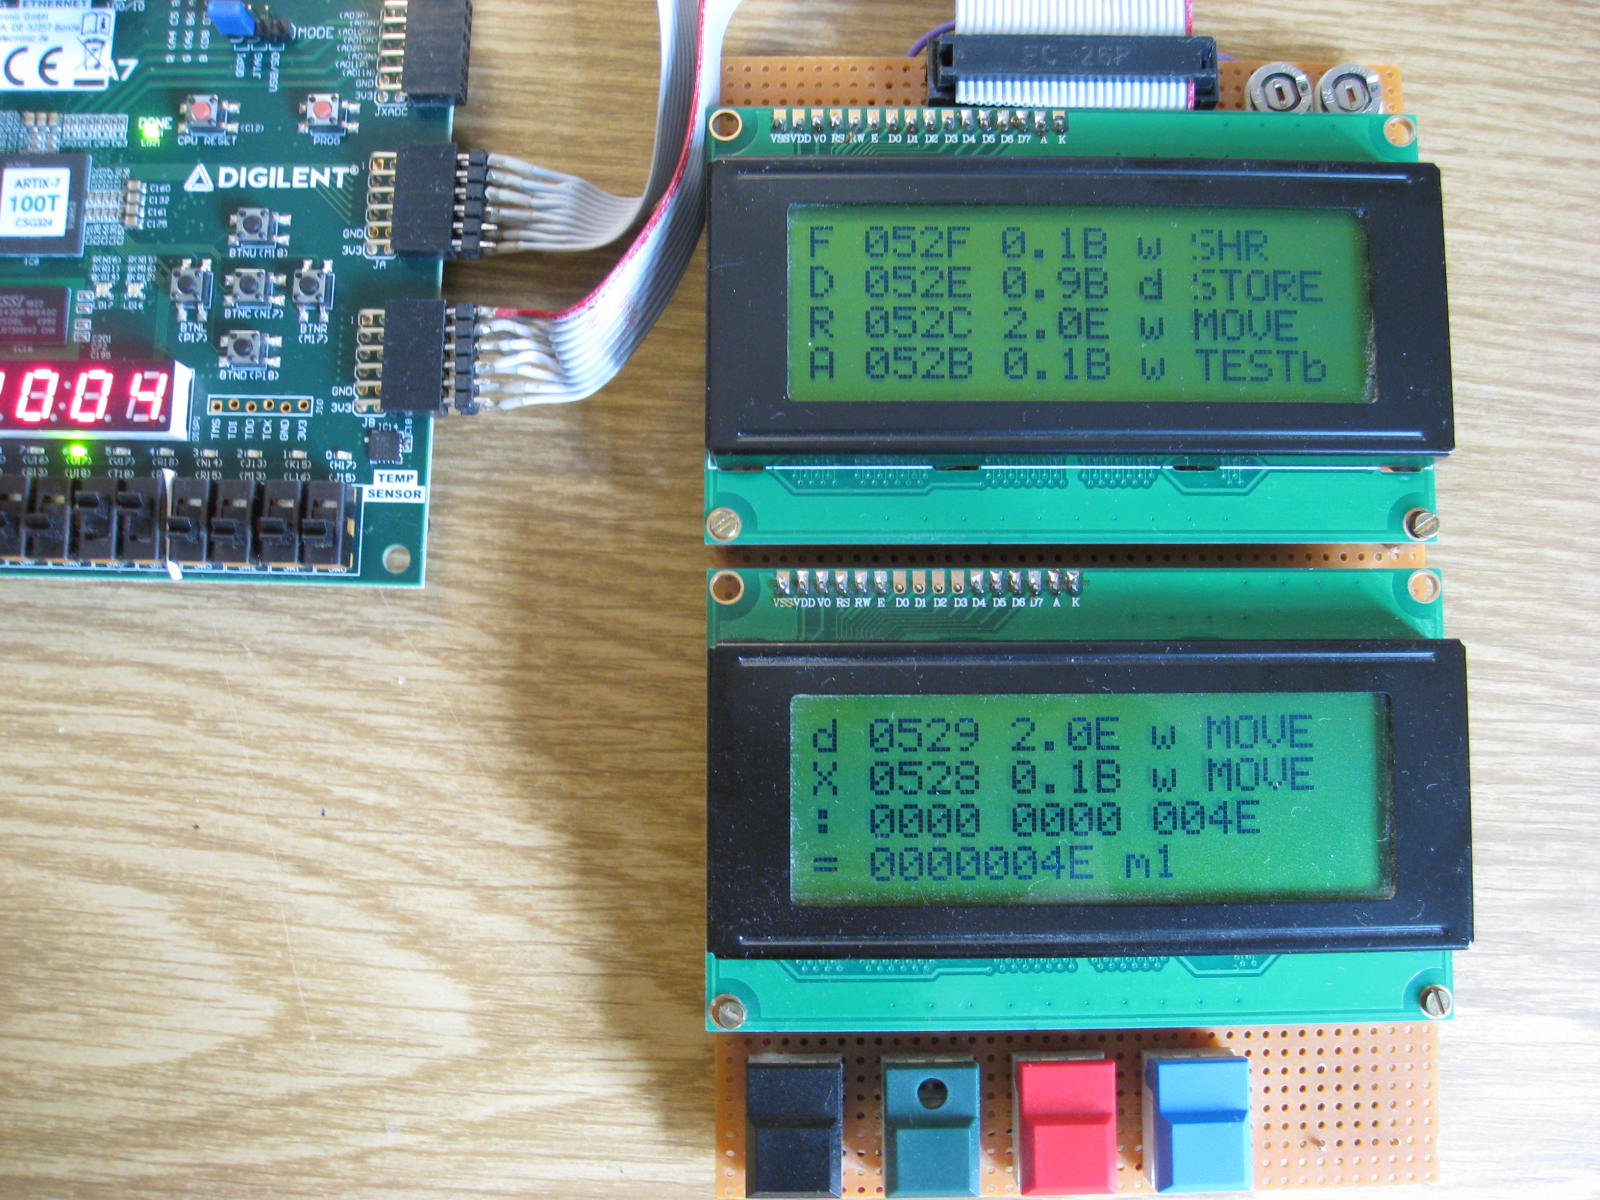
\includegraphics[width=\textwidth]{LCDboard.jpg}
\caption{Prototype add-on board with LCD display and pushbuttons connected to FPGA board}
\label{fig:addOnBoard}
\end{figure}
\end{center}
%\vv
\clearpage


\subsection{Adding external LCD display} \label{Chap:ExternalLCDDisplay}
An external LCD display is useful when debugging. The display shows all stages of the pipeline as well as the result of each instruction during single-stepping. The display has eight lines divided between two four-line LCD modules (see figure \ref{fig:addOnBoard}).
\vv

The components listed in table \ref{table:ComponentListLCD} are needed. 
\vv

\begin{center}
\begin{figure}[ht]
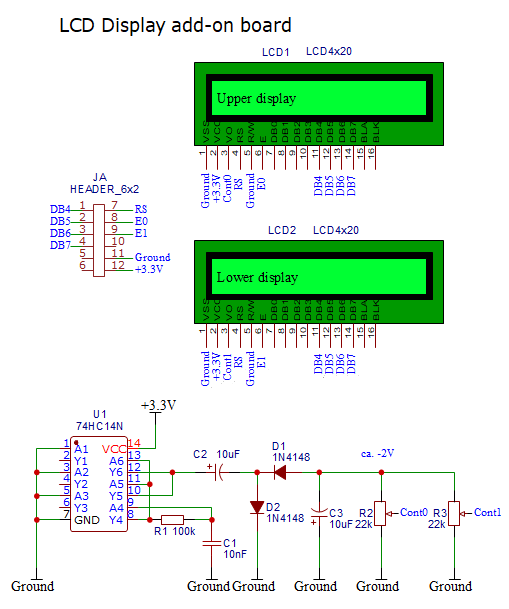
\includegraphics[width=\textwidth]{SchematicLCDdisplay.png}
\caption{Circuit diagram for connecting external LCD display}
\label{fig:LCDdisplayDiagram}
\end{figure}
\end{center}


\begin{table}[h]
\begin{tabular}{|l|l|} 
\hline
\bfseries Component & \bfseries number  \\ \hline
VERO board or similar & 1 \\ \hline
LCD display, 4 lines x 20 columns & 2 \\ \hline
16 pin male pin row for display & 2 \\ \hline
16 pin female connector for display & 2 \\ \hline
2x6 pin male connector & 1 \\ \hline
Smitt trigger 74HC14 or 40106 & 1 \\ \hline
Diode 1N4148 & 2 \\ \hline
Resistor 100 k\Omega & 1 \\ \hline
Trimpot 10 k\Omega{} or 22 k\Omega & 2 \\ \hline
Capacitor 10 nF & 1 \\ \hline
Capacitor 10 \mu{}F & 2 \\ \hline
\multicolumn{2}{|l|}{Component values are not critical} \\ \hline
\end{tabular}
\caption{Component list for external LCD display board}
\label{table:ComponentListLCD}
\end{table}


A circuit diagram for connecting the external LCD display is provided in figure \ref{fig:LCDdisplayDiagram}. Explanation of the diagram: The external LCD display board is connected to the JA socket on the FPGA board. Pin 1-4 on JA are connected to DB4-DB7 on both displays. Pin 7 on JA is connected to RS on both displays. Pin 8 on JA is connected to Enable on the upper display. Pin 9 on JA is connected to Enable on the lower display. Pin 11 and 12 on JA provide ground and +3.3V supply. 
\vv

3.3V is sufficient for the control logic of the LCD displays, but not enough for the backplane voltage. The circuit driven by a 74HC14 Smitt trigger is a charge pump generating a negative voltage for the LCD backplanes. Use the two trimming potentiometers to adjust the contrast on the two display modules.
\vv

\begin{center}
\begin{figure}[ht]
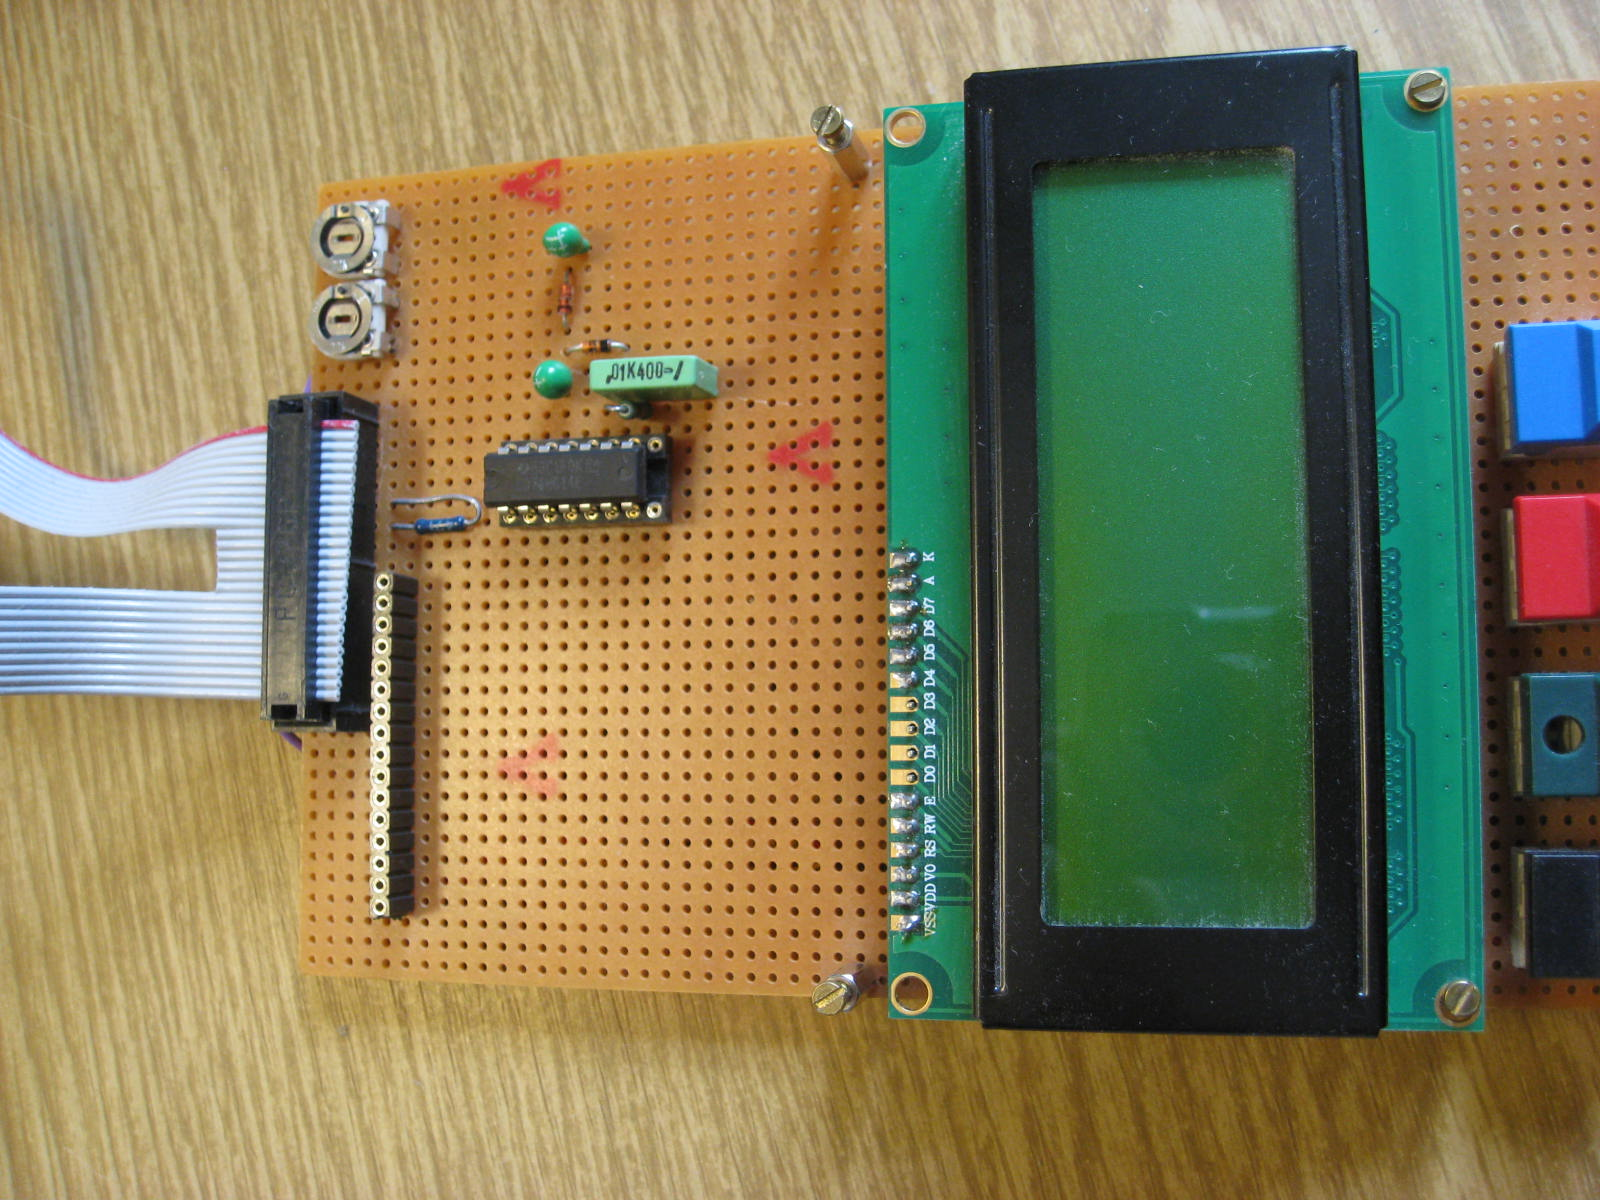
\includegraphics[width=\textwidth]{LCDboardApart.jpg}
\caption{Prototype add-on board with one display removed, showing the underlying components}
\label{fig:AddOnBoardDisassembled}
\end{figure}
\end{center}
\vv


\chapter{Test suite}
A suite of test programs are provided for testing the softcore as well as the emulator. The test programs are written in ForwardCom assembly language.
\vv

The following test programs are currently available:
\begin{itemize}
\item tests\_arithmetics.as: Test all arithmetic instructions with general purpose registers with operand size int8, int16, int32, and int64.
\item tests\_bool\_bit.as: Test boolean and bit manipulation instructions with general purpose registers with operand size int8, int16, int32, and int64.
\item tests\_branch.as: Test jump, call, and branch instructions with general purpose registers with operand size int8, int16, int32, and int64.
\item tests\_formats.as: Test all instruction formats for general purpose registers, including formats for multi-format instructions, single-format instructions, and jump instructions.
\end{itemize}
\vv

The results of the tests are sent via the standard serial output to a terminal. 
\vv

The tests are not fully exhaustive. ForwardCom instructions have an almost infinite number of different variants and special cases. It is impossible to test all combinations of instruction variants and operand values, but the tests are intended to cover as many options and variants as possible.
\vv

The test programs must be linked with the library libc\_light.li if the softcore does not support multiplication, division, push, and pop instructions. 
Example of building a test program:

\begin{lstlisting}

forw -ass -debug=1 tests_arithmetics.as -list=test.txt 
forw -link -debug=1 tests_arithmetics.ex tests_arithmetics.ob libc_light.li
\end{lstlisting}
\vv

See the ForwardCom manual for details about how to use the binary tools.
\vv

The softcore model A 1.00 will obviously fail tests for the instructions that are not supported, i.e. instructions that involve multiplication or division. 
\vv

The tests for operand size int64 will fail for the 32-bit version of the softcore. Instructions that have a fixed operand size of int64 will be shown as working in the 32-bit softcore if the lower 32 bits of the result are correct.
\vv

\chapter{Function library libc\_light.li}
libc\_light.li is a limited version of the standard C library intended for small ForwardCom cores that lack certain instructions. libc\_light.li avoids the use of multiplication, division, push, pop, and sys\_call instructions. Input and output functions are accessing the input and output ports directly rather than using system calls.
\vv

Programs for the softcore model A 1.00 must be linked with libc\_light.li rather than with libc.li.
\vv

The following functions are provided in libc\_light.li:
\vv

\begin{tabular}{|p{25mm}|p{100mm}|p{30mm}|} 
\hline
\bfseries Function name & \bfseries Functionality & \bfseries Source file \\ \hline
\multicolumn{3}{|l|}{Common C functions:} \\ \hline
atoi   & Interpret ASCII string as integer & atoi\_light.as  \\ \hline
atol   & Interpret ASCII string as integer & atoi\_light.as  \\ \hline
getch  & Wait for input from stdin. returns one character & getch\_light.as \\ \hline
getche  & Same as getch, with echo & getch\_light.as \\ \hline
gets\_s  & Read a string from standard input until newline & gets\_light.as \\ \hline
\_kbhit & Return 1 if there is at least one character in the input buffer, 0 otherwise & getch\_light.as \\ \hline
printf  & Print formatted string to stdout & printf\_light.as \\ \hline
sprintf  & Print formatted string to string buffer & printf\_light.as \\ \hline
snprintf  & Same as sprintf, with length limit & printf\_light.as \\ \hline
putchar    & Print a single character to stdout & putchar\_light.as \\ \hline
puts   & Print a string to stdout, append newline & puts\_light.as \\ \hline

\multicolumn{3}{|l|}{Non-standard functions:} \\ \hline

clear\_input  & Clear stdin input buffer & clear\_input\_light.as \\ \hline

divide\_int & Divide two 32-bit signed integers. return quotient and remainder & divide\_int\_light.as \\ \hline

getch\_nonblocking & Same as getch. Does not wait for input. Returns -1 if the input buffer is empty & getch\_light.as \\ \hline

multiply\_int  & Multiplies two 32-bit signed integers. no overflow check & multiply\_int\_light.as \\ \hline

print\_characters  & Prints a very short string to stdout. The input is a 32-bit integer holding up to 4 characters, or a 64-bit integer holding up to 8 characters & print\_characters\_light.as \\ \hline

print\_hexadecimal  & Prints an integer as a hexadecimal number to stdout & print\_hexadecimal\_light.as \\ \hline

print\_integer & Print a 32-bit signed integer as decimal number to stdout & print\_integer\_light.as \\ \hline

print\_string  & Same as puts, does not append newline. Returns a pointer to the first character after the string & print\_string\_light.as \\ \hline

\_entry\_point & This startup code just calls main, unlike the startup code in libc.li that checks for event handlers & startup\_light.as  \\ \hline

\end{tabular}
\vv

The functions printf, sprintf, and snprintf are following the C standard with the following limitations: cannot print floating point numbers, cannot print octal, cannot print decimal integers with more than 32 bits. 64 bit integers can be printed with format "\%lX".
\vv


\chapter{Technical description}

\section{Setting the configuration} \label{SettingConfiguration}
Archive files and precompiled bitstream files for different configurations are provided in \\

\href{https://github.com/ForwardCom/softcoreA/tree/main/deviceA7100T}{github.com/ForwardCom/softcoreA/tree/main/deviceA7100T}:
\begin{itemize}
\item A1T100R32.xpr.zip: Archived project: 32 bit registers. 32 kB data memory. 64 kB code memory.
\item A1T100R32.bit: Bitstream file. 32 bit registers. 32 kB data memory. 64 kB code memory.
\item A1T100R64.xpr.zip: Archived project: 64 bit registers. 32 kB data memory. 64 kB code memory
\item A1T100R64.bit: Bitstream file. 64 bit registers. 32 kB data memory. 64 kB code memory. 58 MHz
\end{itemize}
\vv

Other configurations can be built as follows. 
Change the configuration file config\_A.vh to indicate the desired register size, memory sizes, clock frequency, etc. 
Make sure you set the clock frequency to the value specified in the configuration file. To change the clock frequency, open the Sources window in Vivado, expand the "top" node, double click on clock\_generator, click on the Output Clocks tab, and set the requested output frequency to the desired value.
\vv

The parameters in the configuration files are described here:
\vv
\vv

\textbf{32 or 64 bit registers} \\
The general purpose registers can be 32 or 64 bits. The line\\
\hspace{10mm} \textasciigrave define SUPPORT\_64BIT \\
enables support for 64-bit registers and calculations. Comment out this line for 32-bit registers. The 32-bit configuration is using significantly less hardware resources than the 64-bit version. This has consequences for the maximum clock frequency.
\vv

All calculations work the same with 32-bit registers as with 64-bit registers, except that only the lower 32 bits of a 64-bit result are saved.
\vv
\vv

\textbf{Clock frequency} \\
The CPU clock frequency defined in the line \\
\hspace{10mm} \textasciigrave define CLOCK\_FREQUENCY \\
must match the value set with the clocking wizard.
\vv

The maximum clock frequency depends on the configuration. Differences in register size, memory sizes, and other details influence the maximum clock frequency.  
If you change the configuration, you may need to experiment to find a suitable clock frequency. Vivado will give a warning if the timing requirements cannot be met at the specified clock frequenty. 
\vv 
\vv


\textbf{Serial input and output} \\
The Baud rate for the RS232 serial input and output is defined by the line \\
\hspace{10mm} \textasciigrave define BAUD\_RATE \\
\vv

The serial input and output have queues with power-of-2 sizes defined by the lines \\
\hspace{10mm} \textasciigrave define IN\_BUFFER\_SIZE\_LOG2 \\
\hspace{10mm} \textasciigrave define OUT\_BUFFER\_SIZE\_LOG2 \\
\vv 
\vv


\textbf{Memory sizes} \\
The code memory and data memory have power-of-2 sizes defined by the lines \\
\hspace{10mm} \textasciigrave define CODE\_ADDR\_WIDTH \\
\hspace{10mm} \textasciigrave define DATA\_ADDR\_WIDTH \\
\vv 

The number of entries in the call stack is a power of 2 defined by the line \\
\hspace{10mm} \textasciigrave define STACK\_POINTER\_BITS \\
\vv 
\vv


\textbf{Mask register size} \\
Not all of the bits of a register are needed when the register is used as a mask. In most cases, only one bit is used. We can save hardware resources by not propagating all the bits of a mask register to the execute stage. The number of mask bits to use are defined by the line: \\
\hspace{10mm} \textasciigrave define MASKSZ \\
\vv

This size must be sufficient to contain an instruction tag, i.e. TAG\_WIDTH. More bits may be needed if the mask register contains option bits. A full register size may be needed if the mask register is used for other purposes.
\vv
\vv


\textbf{Instruction tag size} \\
All instructions are identified by a tag when they propagate through the pipeline. The instruction tag must have enough bits to distinguish the maximum number of instructions in flight or pending. This is defined by the line \\
\hspace{10mm} \textasciigrave define TAG\_WIDTH \\
\vv
\vv


\textbf{Loader} \\
The loader is supplied as a file containing the compiled loader code in hex format. The loader file loader.mem is assembled from the source file loader.as and linked with the option -hex2 which makes sure that the loader file is organized with 16 hexadecimal digits (64 bits) per line. 
\vv

The name and maximum size of the loader are defined by the lines \\
\hspace{10mm} \textasciigrave define LOADER\_FILE \\
\hspace{10mm} \textasciigrave define MAX\_LOADER\_SIZE \\
\vv

The loader code is explained in chapter \ref{Chap:Loader}.
\vv
\vv


\section{Hardware in/out connections}
The definition of input and output pins on the FPGA chip are covered by the constraints file Nexys-A7-100T.xdc. This file is based on a template provided by Xilinx and modified to connect the internal signals to specific pins for switches, LEDs, board headers, etc.
\vv

This constraints file is specific for the Nexys A7-100T development board. A different file and different connections are needed for different FPGA models and different development boards.
\vv

A further constraints file, bitstream\_settings\_a.xdc, contains mainly code that is autogenerated by the Vivado tool.
\vv
\vv


\section{Building the code}
The A softcore version 1.00 has been developed with Xilinx Vivado version 2020.1. Note that some versions of Vivado do not support the series 7 FPGAs.
\vv

The Vivado tool is placing source files in a deep and inflexible directory structure that is not very convenient for version control. Therefore, the Github repository includes a zipfile named A1.xpr.zip containing the entire project directory and files as well as all the individual source files. This file was generated with the menu: File $\rightarrow$ Project $\rightarrow$ Archive.
\vv

Users of the softcore will need to unpack the zipfile into an appropriate base directory to get started, and then replace individual source files with any versions that are newer than the zipfile.
\vv

The following source file directories contain files that you may modify or replace with newer versions:\\
\{base\}/A1/A1.srcs/sources\_1/new: verilog files, header files, memory file \\
\{base\}/A1/A1.srcs/constrs\_1/new: device-specific constraints files \\
\vv

All the other directories contain only files generated by the Vivado tool. They should not be modified manually, but may be deleted.
\vv

To rebuild the FPGA bitstream after any modifications, open the project file 
A1.xpr with Vivado. Press the Generate Bitstream icon (green down arrow). This will take approximately 20 minutes. If successful, you can load the new softcore into the FPGA board as described in chapter \ref{Chap:GettingStarted} page \pageref{Chap:GettingStarted}.
\vv

Prebuilt bitstream files for different configurations are provided at Github under devices.
\vv

\subsubsection{Warnings during build}
Vivado produces several warnings during the build process. The following warnings can safely be ignored:
\vv

\begin{itemize}
\item {}[Netlist 29-345] The value of SIM\_DEVICE on instance 'clock\_generator\_inst/inst/clkout1\_buf' of type 'BUFGCE' is 'ULTRASCALE'; ... source netlist. 

\item {}[Designutils 20-4072] Reference run did not run incremental synthesis because the design is too small; reverting to default synthesis

\item {}[Constraints 18-5210] No constraints selected for write...

\item {}[Power 33-332] Found switching activity that implies high-fanout reset nets being asserted for excessive periods of time which may result in inaccurate power analysis.

\item {}[Vivado 12-1017] Failed to delete one or more files in run directory .../A1/A1.runs/synth\_1

\item {}[Synth 8-6841] Block RAM (ram\_reg) originally specified as a Byte Wide Write Enable RAM cannot take advantage of ByteWide feature and is implemented with single write enable per RAM

\item {}[Synth 8-7129] Port instruction\_in[29] in module ... is either unconnected or has no load

\item {}[DRC DPOP-1] PREG Output pipelining: DSP muldiv\_inst/p\_0\_out output ... is not pipelined...

\end{itemize}
\vv

You may disable unwanted warnings because it creates a risk that other warnings are overlooked. Warnings other than these may indicate serious problems.
\vv

Occasionally, Vivado fails without any diagnostic message. The problem usually goes away when making any change in the code. A safe way to make changes is to comment out or in some debug signals in the file debugger.vh.
\vv


\subsubsection{Timing problems}
When building a modified softcore, it often happens that it fails to meet the timing requirements. The Vivado tool is not always able to find an optimal routing pattern. Small changes in the code may result in a different routing pattern that is either faster or slower. If only a few signal paths fail to meet the timing requirements by a small negative slack, then it is possible that the problem will go away after any small change in the code, for example in the debug signals or the number of bits in the mask register.
\vv

If the timing problem is more severe, then you need to redesign the code that is causing the problem, or lower the clock frequency.
\vv

\section{Description of the hardware code} \label{Chap:DescriptionHWCode}
The hardware code for the ForwardCom softcore is written in the hardware description language SystemVerilog. 
\vv

The CPU is based on a Harvard architecture with separate code memory and data memory that can be accessed simultaneously. There is write access to the code memory for the sake of the on-chip loader, but it is not possible to read from the code memory by other means than fetching code.
\vv

The CPU design has six pipeline stages:
\vv

\begin{enumerate}
\item Fetch
\item Decode
\item Register read
\item Address generation
\item Data read
\item Execute
\end{enumerate}
\vv

Instructions are propagating one by one through the pipeline, advancing one stage per clock cycle.
\vv

The hardware design consists of modules. Each pipeline stage is a module. In addition to this, there are modules for code memory, data memory, call stack, input/output, etc. Each module has registers (D flip-flops) on its outputs, but not on its inputs. This means that it takes one clock cycle to send a signal from one module to another. The complexity within each module is limited to what can be completed in one clock period.
\vv

The following is a detailed description of each pipeline stage and each module.
\vv

\subsection{Fetch stage}
The fetch stage in the pipeline will fetch code from the code memory at a rate of two words (64 bits) per clock cycle from even addresses. The code words are loaded into a buffer with a size of 8 words.
\vv

While dispatching one instruction to the decode stage, the fetch unit is looking at the next instruction in the buffer in order to identify jump, call, and return instructions as early as possible. The ISA is designed so that these instructions can be identified easily. Direct, unconditional jump and call instructions with a 24-bit relative address are handled immediately by the fetch unit so that the target instruction can be loaded from the code memory with a delay of only one clock cycle. Return instructions are handled equally fast, using a prefetched return address from the call stack. This is possible only because the call stack and data stack are separate and independent.
\vv

Conditional jumps, indirect jumps and calls, and any other control transfer instructions have to go through the pipeline. In this case, the fetch unit has to wait for a target address from the ALU. This is causing a delay of 7 clock cycles for taken jumps. Not-taken conditional jumps are one clock faster because the target is already in the code buffer.
\vv

The fetch unit is sending a return address to the call stack for all kinds of call instructions.
\vv

It takes two clock cycles to fetch code from the code memory: one clock cycle for sending the address to the code memory, and one clock for getting the result back to the fetch unit. The fetch unit keeps prefetching code from the next address as long as the code buffer is not full. A shift register named next\_underway keeps track of whether the next code words are underway from the code memory. Another shift register target\_underway does the same after a jump. Jump addresses are fed directly from the ALU to the code memory in order to save one clock cycle.
\vv

A reset signal will cause a jump to the start address of the loader. A restart signal will cause a jump the the restart address which is the loader address plus 1.
\vv

\subsection{Decode stage}
The decoder identifies the instruction format, category, number of operands, register use, result type, etc. It also assigns a unique tag to identify each instruction in the pipeline.
\vv

The decode stage includes a state machine for push and pop instructions that generate multiple micro-operations. The fetch unit is stalled until all the necessary micro-operations have been dispatched to the next stage in the pipeline. The number of different instructions that generate multiple micro-operations should be kept at a minimum in order to limit the complexity of the decode stage.
\vv

The outputs from the decoder includes the variables listed below. Possible values for each variable are defined in the configuration file, described on page \pageref{SettingConfiguration}.
\vv

\begin{itemize}
\item vector\_out: 1 if vector instruction
\item category\_out: single format, multiformat, or jump instruction
\item format\_out. Instruction format A, B, C, E
\item rs\_status\_out. Use of RS register field: source register, vector, pointer, etc.
\item rt\_status\_out. Use of RT register field: source register, vector, index, vector length
\item ru\_status\_out. Use of RU register field: source register, vector
\item rd\_status\_out. Use of RD register field: source register, vector
\item mask\_status\_out. Use of mask register field: source register, vector
\item mask\_options\_out. Mask may contain option bits (floating point only)
\item mask\_alternative\_out. Mask register and fallback register used for alternative purposes
\item fallback\_use\_out. Which register is used for fallback
\item num\_operands\_out. Number of source operands. 0 - 3
\item result\_type\_out. Type of result: normal register, system register, memory, other
\item offset\_field\_out. Size of memory address field
\item immediate\_field\_out. Size of immediate operand field
\item scale\_factor\_out. Scale factor for array index
\item index\_limit\_out. Array index has a limit
\end{itemize}
\vv


\subsection{Register read stage}
The register file is included in the same module as this pipeline stage so that it is possible to read register values without delay. This includes the 32 general purpose registers as well as the numeric control register (NUMCONTR), data pointer (DATAP), and thread data pointer (TRHEADP), but not other system registers.
\vv

All registers needed by an instruction are read at this stage, and the values are propagated through the pipeline to the stage where they are needed, i.e. the address generation stage or the execution stage.
\vv

The instruction tag is written to the destination register in the register file. This indicates to subsequent instructions that the value of this register is not available yet. The tag identifies the instruction that is going to deliver the value. Subsequent stages in the pipeline must monitor the result buses for results marked with the tag of any missing register value. The tag is then replaced by the new value and propagated through the rest of the pipeline. 
This mechanism may be considered a form of register renaming. Multiple values of the same logical register can be in flight in the pipeline at the same time. The tag of a missing register value is replaced by the actual value as soon as it appears on one of the result buses. All stages in the pipeline after the register read stage are monitoring the result buses for missing register values.
\vv

Each entry in the register file includes an extra bit which is 1 if the file contains a tag for a pending value, or 0 if the file contains the actual value of the register. The same applies to values propagating through the pipeline.
\vv

It is important that tags are written to the register file in the same pipeline stage as all register reads. This makes sure that we get the correct version of a changing register.
\vv

The register read stage is sending the values or tags of up to five registers, including a mask register, to the address generation stage in the pipeline.
\vv


\subsection{Address generation stage}
The address generator calculates the address of a memory operand. 
All memory addresses are relative to a base pointer, which may be a general purpose register, DATAP, THREADP, or IP. 
The address may consist of three components: A base pointer, a scaled array index, and a constant offset. A base pointer register is always present, the other components are optional.
\vv

The address generator sends the calculated address of a memory operand to the data memory for any instruction that involves memory read or write. Memory read and memory write operations are initiated in the same pipeline stage so that a memory read never has to wait for a preceding write.
\vv

The address generator needs to wait for any missing register value needed for base pointer, array index, vector length, or a value to write. This will generate stalls in the preceding pipeline stages and bubbles in the subsequent pipeline stages whenever a needed register value is not available yet.
\vv

Testing the validity of the calculated memory address should ideally be implemented in this stage, but unfortunately this leads to timing problems because the address calculation involves two additions. An extra compare operation after the two additions is difficult to fit into the time slot of a single clock period. Therefore, the detection of memory access violations is currently postponed to the next pipeline stage.
\vv

The address generation stage does some additional decoding in parallel with the address calculation. It sorts the source operands of the instruction according to the order of priority defined by the ForwardCom standard: 
immediate operand, memory operand, RT register, RS register, RU register, RD register. Up to three source operands are taken from the fields defined by the instruction format according to this order of priority, with the last operand first. Immediate operands are identified and sign-extended or uncompressed if needed. The values of all operands are sent to the next pipeline stage as operand1\_out, operand2\_out, and operand3\_out if the values are available. The output memory\_operand\_out indicates that one source operand is a memory operand that will be available after two clock cycles.
\vv

\subsection{Data read stage}
The main purpose of the data read stage is to wait one clock cycle for the value of a memory operand to arrive from the data memory. Normally, the value of a memory operand will arrive just in time for the execution stage to use it. However, the data read stage can catch and store the value in case the instruction is delayed by a pipeline stall. The data read stage also checks if a memory address is valid. 
\vv

The operation to do in the execution stage is identified in the data read stage and indicated by the variable opx\_out. The operation for multiformat instructions is identified by the OP1 field only so that opx\_out = OP1.
\vv

Some single-format instructions are short forms of instructions that also exist in multiformat versions. These instructions are translated to the multiformat equivalents in opx\_out. Single-format instructions that do not have a multiformat equivalent are given a unique value of opx\_out.
\vv

Branch instructions are split into the corresponding ALU operation, such as "add" or "compare" in opx\_out, and the branch condition indicated by opj\_out.
\vv

The operand type ot\_out is identified for instruction formats that do not have an operand type field.
\vv

The data read stage decides which module to use for the execution stage. This is indicated by exe\_unit\_out.
\vv


\subsection{Execution stage, ALU}
The ALU module implements the execution stage for most integer instructions, such as addition, bit operations, shift, branch, etc. The latency is one clock cycle for all these instructions.
\vv

This is the most critical pipeline stage in terms of timing, and the one that determines the maximum clock frequency. This includes three critical steps:
\begin{enumerate}
\item Input multiplexers. Retrieve each source operand value from either the previous pipeline stage (propagated value), from one of the result buses if the value was output in the preceding clock cycle, or directly from data memory. Data memory values with a size less than 64 bits must be selected from any position within a 64-bit memory line.
\item Do the actual calculation or operation
\item Cut off the result to the desired operand size, or replace it with a fallback value in case the mask is zero
\end{enumerate}
\vv

The result is output to result bus 1 as result\_out together with register\_a\_out that identifies the destination register, and tag\_val\_out that indicates the instruction tag.
\vv

Jump and branch instructions have the additional outputs jump\_out and nojump\_out, indicating whether a branch is taken or not, and jump\_pointer\_out that gives the address of the jump target in case the jump is taken.
\vv

The ALU module contains several general units that can service more than one instruction each. This includes a compare unit that is used for signed and unsigned compare instructions, max, min, and compare/branch instructions. A bit manipulation unit for bit operations such as clear, set, toggle, test, etc. A barrel shifter for all shift, rotate, and move\_bits instructions. And a bit scan module for bitscan and roundp2 instructions. There are also several single-purpose units.
\vv

The bitscan instruction appears to be particularly critical in terms of timing. Future implementations may move the bitscan instruction to a unit with a longer latency.
\vv


\subsection{Execution stage, in\_out\_ports}
The in\_out\_ports unit implements the execution stage for interfaces to external communication as well as several capabilities registers, performance counters, etc.
\vv

The RS232 serial interface consists of a UART receiver, a UART transmitter, and FIFO buffers on both input and output.
\vv

System registers that can be renamed, i.e. NUMCONTR, DATAP, and THREADP, are accessed in the register read stage, while all other system registers are implemented or accessed in the in\_out\_ports module. Some of these registers are read-only, while others can also be written or reset. It is necessary that read and write of the same register happens in the same pipeline stage.
\vv

Register results are output to result bus 1 in the same was as for the ALU unit. The instruction latency is one clock cycle.
\vv

\subsection{Execution stage, mul\_div}
The mul\_div unit implements the execution stage for instructions that have a latency higher than one, such as multiplication and division. The result is output to result bus 2.
\vv

The latency for multiplication and mul\_add is 5 clock cycles. Multiplication is pipelined so that a new multiplication can start every clock cycle if the operands are ready. 
\vv

Division is using a radix-4 division loop that is using one clock cycle for every two significant bits of the result. Two clock cycles are used before the division loop for sign detection and for shifting the divisor to the highest position that is not higher than the dividend. One clock stage is used after the division loop for rounding the result, adjusting the sign, etc. The rem instruction is using the same mechanism. 
Division is not pipelined. The main pipeline will be stalled if a division instruction is waiting for a previous division to finish.
\vv


\subsection{Pipeline synchronization signals}
There are no instruction queues between the pipeline stages. This means that if one pipeline stage is waiting for an operand that is not available yet, then all preceding pipeline stages must stand still and keep their data until the next pipeline stages are ready to receive a new instruction. This is called a pipeline stall. While one pipeline stage is waiting for an operand, all subsequent pipeline stages will be idle. This is called a pipeline bubble.
\vv

There are three units that can cause pipeline stalls and bubbles in the present design:
\vv

\begin{enumerate}
\item The fetch unit is waiting for an instruction to be fetched from the code memory after a jump or after the code buffer has been exhausted by multiple triple-size instructions. This is causing a bubble to propagate through the entire pipeline
\item The address generation stage is waiting for a register value needed for the address calculation. This is causing a stall in the preceding pipeline stages and a bubble in the subsequent stages
\item The execution stage is waiting for the value of a register operand. This is causing a stall in the entire pipeline. This also happens if a division instruction is waiting for the division unit to be vacant.
\end{enumerate}
\vv

The handling of pipeline stalls and bubbles is quite tricky and delicate because stalls must be predicted one clock cycle in advance, and we must make sure that every instruction is dispatched once, and only once, from each pipeline stage to the next. The dataread stage is sending out predict\_tag signals giving the instruction tag of the result that is predicted to be sent to result bus 1 in the next clock cycle. The predict\_tag signal is used by the register read stage to predict whether the necessary register values will be available for the address calculation stage in the next clock cycle. In the same way, the data read stage is using the predict\_tag signal to predict whether all operands will be ready for the execution stage in the next clock cycle. The mul\_div unit is sending out a predict\_tag2 signal one clock cycle before a result is sent to result bus 2.
\vv

The register read stage and the data read stage will send out a stall\_predict signal if they predict a stall in the next clock cycle. These signals are fed to stall\_in inputs of all preceding pipeline stages, telling them to halt and keep their data until the pipeline is ready to proceed.
\vv

A stalled pipeline stage must keep all its data unchanged, with one exception. It must watch the result buses for any results that match a missing register value for the contained instruction. 
\vv

Pipeline bubbles are controlled by valid\_in and valid\_out signals. The valid\_out signal of each pipeline stage is connected to the valid\_in signal of he next stage. This signal is 1 if a valid instruction is being propagated, or 0 if there is a pipeline bubble. All other inputs must be ignored when the valid\_in signal is zero.
\vv


\subsection{Data memory}
The module named data\_memory contains a RAM memory for data only. The size is a power of 2 determined by the variable DATA\_ADDR\_WIDTH defined in a configuration file.
\vv

The data RAM has one read port and one write port, each 64 bits wide. Reads and writes of less than 64 bits are allowed, but all reads and writes must have natural alignment.
\vv

The input read\_data\_size indicates data sizes of 8, 16, 32, or 64 bits. Reads of less than 64 bits are right-justified in the output read\_data\_out.
\vv

The 64-bit input write\_data\_in is divided into eight bytes enabled separately. The 8-bit input write\_enable enables each byte separately. Memory writes of less than 64 bits are controlled by the address generator by placing the data in the right position and enabling only the bytes that contain actual data.
\vv


\subsection{Code memory}
The module named code\_memory contains a memory for code only. The size is a power of 2 determined by the variable CODE\_ADDR\_WIDTH defined in a configuration file.
\vv

The code memory has one read port that is 64 bits wide. Unaligned reads are not possible. A read of a 32-bit word from an odd address must be implemented as a 64-bit read from the preceding even address.
\vv

The code memory has one write port that can accept 64-bit writes to an even address or 32-bit writes to an even or odd address. The write port is intended for the loader only.
\vv

A loader can be placed in the top of the code memory. A hex file with a name defined by LOADER\_FILE is placed at an address calculated as the end address of the code memory minus MAX\_LOADER\_SIZE. This file must be organized as 64-bit lines.
\vv


\subsection{Call stack}
The call stack is used for function return addresses only. The size is a power of 2 determined by the variable CALL\_STACK\_POINTER\_BITS defined in a configuration file.
\vv

The call stack is accessed by the instruction fetch unit only. A return address is pushed on the call stack when a call instruction is detected, and popped from the call stack when a return instruction is detected. The call stack cannot be accessed by data push and pop instructions.
\vv

Return addresses are communicated via the push\_data input and the pop\_data output. The value of pop\_data is prefetched in advance so that it can be accessed immediately by the fetch unit. The value of pop\_data is valid one clock cycle after a push or pop operation. Therefore, there must be a one clock cycle delay between a call or return and the next return. This is not a problem in the current design because the fetch unit has a delay of at least one clock cycle after any call or return anyway.
\vv


\subsection{Debug displays}
There are two debug displays as explained in chapter \ref{Chap:Debugger}. A LED display on the FPGA board, and an optional LCD display on an add-on board.
\vv

The LED display is controlled by a Verilog header file, debugger.vh. This file is included in the top module so that it has direct access to all global signals. Local signals inside a module are accessed through debug outputs from the module in questions. You may modify the file debugger.vh to get access to a particular signal. debugger.vh includes an instance of a 7-segment display driver seg7.sv. The debugger writes an error code in the 7-segment LED display instead of the selected debug information in case of a runtime error.
\vv

The external LCD display is driven by the module debug\_display. 
It includes an instance of an LCD driver named lcd. 
The LCD driver contains a state machine that writes to the LCD displays, sending 4 bits at a time.
\vv

The debug\_display module writes information about the contents of each pipeline stage to the LCD displays. The debug\_display module has only access to the outputs of each module. Source operand values in the execute stage are reconstructed inside the debug\_display module rather than transferred from the execute modules. The translation of operation codes to opx, that occurs in the data read stage, is mirrored inside the debug\_display module for the display of pipeline stages prior to the data read stage. This allows the debug display to write the names of instructions in all pipeline stages.
\vv

The debug\_display module has internal registers on most signals to avoid timing problems and to diminish restrictions on signal routing. It is no problem that the data are delayed a few clock cycles because the LCD display is only useful during single-stepping.
\vv


\subsection{Top module}
The top module is instantiating the pipeline stages and other modules and making the connections between them.
\vv

Input and output connections to external devices are defined by the top module.
\vv


\subsection{Byte based and word based addresses}
Read and write address signals for the data memory are absolute addresses with byte granularity. Address signals for the code memory have word granularity (4 bytes) and are relative to the start of the code memory. The same applies to the instruction pointer.
\vv

Translation from word addresses to byte addresses occurs in the address generator when calculating an address relative to IP. Translation from byte addresses to word addresses occurs in the ALU when executing an indirect jump, and in the code memory module when writing to the code memory (only the loader should write to code memory).
\vv


\section{Loader} \label{Chap:Loader}
The loader is a piece of software written in ForwardCom assembly language. The loader can load an executable program (.ex file) into the program memory and data memory. The source code for the loader is in the file loader.as. 
\vv

The loader is placed at the end of code memory. The start address of the loader is calculated as the size of the code memory minus MAX\_LOADER\_SIZE. This address is hard-coded into the softcore. The CPU will jump to this address at start and when the load button is pressed. 
\vv

The loader can be debugged by inserting breakpoint instructions at the desired places. It is recommended to set  MAX\_LOADER\_SIZE to a multiple of 0x100 during debugging so that the last two digits of addresses on the debug display match addresses in the loader assembly listing.
\vv

A loaded program can be re-started by jumping to the RESTART code, which is placed at the loader start address plus 1.
\vv

The loader works as follows. The user uploads the desired program as an executable file (.ex file). The loader starts reading the .ex file through the RS232 serial interface. The first part of the .ex file contains a file header and program headers, according to the official ForwardCom definition in the file elf\_forwardcom.h. These headers are read into the beginning of data RAM and analyzed to find code sections, const data sections, and data sections. The raw data of these sections are then read and placed in code memory and data memory. The program memory starts at an address immediately following the end of data memory. Program code sections are placed in code memory. 
Constant (read-only) IP-based data sections are placed at the end of data RAM so that they can be addressed relative to the instruction pointer, IP.
\vv

Data sections with read/write access are read into the first vacant data RAM address and later moved down to address zero when the loader has finished using the program headers. The rest of data RAM is then cleared to zero.
\vv

The data stack pointer (r31) is set to the top of vacant data RAM, which is the beginning of const data. The program start address, DATAP, and THREADP are set to the addresses defined in the file header. These addresses are not stored in data RAM, but inserted in the RESTART code so that all data RAM is available to the running program. When the loader has finished loading all sections, it jumps to the RESTART code. The RESTART code sets the stack pointer, DATAP, and THREADP, clears all other registers, and jumps to the program start address. 
\vv

The RESTART code clears the registers but does not reset the RAM memory when the restart button is pressed.
\vv

The loader works with both the 32-bit version and the 64-bit version of the softcore.
\vv 

The loader assumes that the .ex file is fully position-independent. It is not able to relocate code containing absolute addresses.
\vv


\section{Resource use}
This section discusses how different aspects of the softcore design affects the use of hardware resources.
\vv

The use of LUTs (lookup tables) and registers (flip flops) in the 32-bit and 64-bit configurations are listed in table \ref{table:ResourceUse}.

\begin{table}[h]
\begin{tabular}{|l|l|l|l|l|} 
\hline
\bfseries Module & \multicolumn{2}{|c|}{\bfseries Slice registers} & \multicolumn{2}{c|}{\bfseries Slice LUTs}  \\
\bfseries  & \bfseries 32-bit version & \bfseries 64-bit version & \bfseries 32-bit version & \bfseries 64-bit version  \\ \hline
Fetch                &  347  &  347  &  1214 &  1188 \\ \hline
Decode               & 242   &  257  &   571 &   675 \\ \hline
Register read        & 1635  & 3014  &  2859 &  5416 \\ \hline
Address generator    & 509   &  734  &   895 &   517 \\ \hline
Data read            & 258   &  375  &  3129 &  6040 \\ \hline
Execute ALU          & 84    &  119  &  1005 &  2649 \\ \hline
Execute in/out, uart & 698   & 1205  &   477 &   571 \\ \hline
Execute mul/div      & 517   &  939  &  1593 &  2389 \\ \hline
Code memory          & 0     &    0  &    44 &    44 \\ \hline
Data memory          & 3     &    3  &   263 &   291 \\ \hline
Call stack           & 29    &   29  &   443 &   445 \\ \hline
Debug display        & 485   &  487  &   735 &   778 \\ \hline
Total                & 4990  & 7392  & 13248 & 21121 \\ \hline
\end{tabular}
\caption{Resource use of softcore}
\label{table:ResourceUse}
\end{table}
\vv

The propagation of source operand values through the pipeline is using 32 or 64 bits per operand in each pipeline stage. If a pipeline stage is stalled, then it needs to keep the old instruction on its output until the next stage is ready to receive it. At the same time, it needs to catch operand values from the result buses for the pending next instruction. This doubles the required number of registers in the register read and address generator stages. If we allow three source operands and a mask of 64 bits each, then we need 4*64*2 = 512 flip flops just for catching and propagating data in each pipeline stage. This number of flip flops is not a problem for an FPGA with 100,000 cells or more, but the associated logic and routing is actually consuming a significant amount of resources. We may reduce the resource use for smaller applications by reducing the register size to 32 bits. The mask register may be reduced to 16 bits.
\vv

The result buses are also consuming a significant amount of resources because each pipeline stage must monitor all result busses and compare the result tags with all four source operands (including mask register). This is particularly critical in the execution stage where timing is critical. 
Therefore, we have multiple execution units sharing the same result busses.
\vv

The timing problems that we encounter are often dominated by routing delays rather than logic delays. It is necessary to take this into account and limit the number of cross connections between modules.
\vv

An important feature that distinguishes ForwardCom from other ISAs is that each instruction can have many different variants. This feature is actually fairly cheap in terms of hardware resources. There are many different instruction formats, and it takes many lines of verilog code to decode these formats, but the resulting hardware is actually a fairly trivial combinational logic with a limited number of inputs and outputs. It requires only a few bits to tell where an operand is or what a register is used for -- in contrast to the many bits used for handling and propagating up to three or four operands of 64 bits each. The timing of the decoding process is not critical at all because the logic to handle all aspects of the decoding process can be divided over several pipeline stages. Likewise, we have several pipeline stages to handle the decoding and unpacking of immediate constants and option bits, and it is not important which pipeline stage we place this code in.
\vv

The fact that ForwardCom has instructions that combine memory read with arithmetic or logic instructions comes at a significant price, though, because it makes the pipeline longer. 
\vv


\section{Future development}
This section discusses some prospective future extensions to the ForwardCom softcore.
\vv

Vector instructions will be implemented with a separate pipeline for each 64-bit vector lane. Each lane will have its own register file holding a 64-bit slice of each vector register. Designs with small vectors may have direct access to a common data RAM. Designs with long vectors may have one data cache or RAM for each vector lane. Memory access will be fast when aligned by the maximum vector length but slower when not aligned because it requires a very big barrel shifter to exchange data between lanes. The vector pipeline probably needs an extra stage for data alignment.
\vv

A superscalar softcore will be able to fetch and decode two or more instructions per clock cycle. There may be two pipelines for non-vector instructions: One for instructions with memory operands, and a shorter pipeline for instructions without memory operands. There will probably be only one pipeline for vector instructions. It will be possible to execute two instructions per clock cycle if they can go to two different pipelines. The short pipeline for instructions without memory operands will make jump delays shorter. The instructions will be executed in order within each pipeline.
\vv


\section{Performance metrics}
The maximum clock frequency varies from 50 to 70 MHz depending on register size, memory sizes, and other configuration details. The current settings are 64 MHz for the 32-bit register version and 56 MHz for the 64-bit register version of the softcore. The maximum clock frequency can be increased by a few MHz when the memory sizes are reduced or some instructions removed from the ALU. The bitscan instruction, in particular, is critical.
\vv

The maximum throughput is one instruction per clock cycle. The latency is one clock cycle for most instructions. 
\vv

Multiplication and mul\_add instructions have a latency of five clock cycles and a throughput of one multiplication per clock cycle. Division has a latency of three clock cycles plus one additional clock cycle for every two significant bits in the result. It is not possible to start a new division before a previous division is finished. Push and pop instructions take one clock cycle for each register plus a single additional clock cycle for adjusting the stack pointer. All other arithmetic and logic instructions have a latency of one clock cycle.
\vv 

Unconditional direct jumps, calls, and returns have a latency of 2 clock cycles.
\vv

Conditional jumps have a latency of 7 clocks when taken and 6 clocks when not taken. Indirect and multiway jumps and calls have a latency of 7 clocks.
\vv

Memory reads have a delay of 2 clocks after the modification of a pointer or index register that is needed in the address calculation. There is no delay for memory reads if address registers are not modified in the preceding two instructions.
\vv

Memory writes have a delay similar to memory reads if address registers are modified within the preceding two instructions. The same delay applies if the register holding the value to write is modified within the preceding two instructions.
\vv

All instructions start to execute in order, but they do not necessarily finish in order in case of instructions with longer latencies. Two instructions can finish in the same clock cycle, using different result buses.
\vv


\section{Portability}
The hardware code written in SystemVerilog avoids device-specific code. It should be possible to port this to other FPGA models, other FPGA brands, or even to an ASIC.
\vv

The clock generator is auto-generated by the Vivado clock vizard. It needs to be adjusted or redesigned for other FPGAs.
\vv

The multiplication unit may need different latencies for different FPGA types. This is adjusted by the value of MUL\_STEPS in the file mul\_div.sv. Some FPGA types may supply library code for faster division, but the code provided in mul\_div.sv is written to be generic and device-independent.
\vv

The 7-segment display on the Nexys A7 FPGA board is used for debugging and error messaging. Other FPGA boards may have other kinds of display.
\vv

The constraints files contain device-specific information about pin connections etc. The connections to external devices need to be redesigned for other FPGAs.
\vv


\section{File list}
The following files are provided with the soft core:

\begin{table}[h]
\label{table:FileList}
\begin{tabular}{|l|l|} 
\hline
\bfseries File & \bfseries Explanation  \\ \hline
top.sv & top level hardware description file, system verilog \\ \hline
fetch.sv & pipeline stage 1: instruction fetch \\ \hline
decoder.sv & pipeline stage 2: instruction decoder \\ \hline
register\_read.sv & pipeline stage 3: register file \\ \hline
addressgenerator.sv & pipeline stage 4: address calculation \\ \hline
dataread.sv & pipeline stage 5: data read \\ \hline
alu.sv & pipeline stage 6: execution unit for most arithmetic and logic instructions \\ \hline
mul\_div.sv & pipeline stage 6: execution unit for multiplication and division \\ \hline
in\_out\_ports.sv & pipeline stage 6: execution unit for input, output, system registers, etc. \\ \hline
uart\_and\_fifo.sv & UART and FIFO buffers used by input and output ports \\ \hline
code\_memory.sv & code memory \\ \hline
data\_memory.sv & data RAM \\ \hline
call\_stack.sv & call stack for function return addresses \\ \hline
debouncer.sv & debouncer for on-board pushbuttons \\ \hline
debugger.vh & on-board 7-segment debug display \\ \hline
seg7.sv & 7-segment display decoder for on-board display \\ \hline
debug\_display.sv & add-on board LCD debug display \\ \hline
lcd.sv & LCD display driver \\ \hline
config\_A.vh & configuration file, defining register size, memory size, etc. \\ \hline
defines.vh & definition of constants \\ \hline
subfunctions.vh & subfunctions used by ALU \\ \hline
loader.mem & hex file for on-board loader \\ \hline
loader.as & assembly source code for on-board loader \\ \hline
manual/softcore\_A.pdf & this manual \\ \hline
manual/softcore\_A.tex & Latex source for this manual \\ \hline
\end{tabular}
\end{table}
\vv


\chapter{Revision history}

\subsubsection{Version A1.01, 2022-12-29}
\begin{itemize}
\item Revision for ForwardCom standard version 1.12. Multiplication, division, push, and pop instructions added.
\end{itemize}

\subsubsection{Version A1.00, 2021-08-07}

\begin{itemize}
\item First published ForwardCom softcore. 32 and 64 bit versions. Integer only. No vectors.
\end{itemize}
\vv


\chapter{License}
The hardware description code is published under the \href{https://cern-ohl.web.cern.ch/}{CERN Open Hardware License weakly-reciprocal}, version 2 or later. This is a license for hardware similar to the Gnu General Public License for software. 
\vv

All the code is written from scratch without importing any code from elsewhere. This makes sure that all the code has the same license.
\vv

This manual is copyrighted 2021-2022 by Agner Fog with a 
\href{https://creativecommons.org/licenses/by/4.0/legalcode}{Creative Commons license CC-BY}.


\end{document}
